\documentclass[12pt,a4paper]{article}

% Essential packages
\usepackage[utf8]{inputenc}
\usepackage[T1]{fontenc}
\usepackage[english]{babel}
\usepackage{geometry}
\usepackage{graphicx}
\usepackage{xcolor}
\usepackage{fancyhdr}
\usepackage{titlesec}
\usepackage{tocloft}
\usepackage{booktabs}
\usepackage{amsmath}
\usepackage{amssymb}
\usepackage{listings}
\usepackage{hyperref}
\usepackage{caption}
\usepackage{subcaption}
\usepackage{enumitem}
\usepackage{float}
\usepackage{colortbl}
\usepackage{pgfgantt}

% Page geometry
\geometry{
    top=2.5cm,
    bottom=2.5cm,
    left=2.5cm,
    right=2.5cm,
    headheight=15pt
}

% Color definitions
\definecolor{primaryblue}{RGB}{41, 128, 185}
\definecolor{secondaryblue}{RGB}{52, 152, 219}
\definecolor{darkgray}{RGB}{44, 62, 80}
\definecolor{lightgray}{RGB}{149, 165, 166}
\definecolor{accentgreen}{RGB}{39, 174, 96}
\definecolor{codebackground}{RGB}{248, 249, 250}

% Define team member colors
\definecolor{JesusGreen}{HTML}{27ae60}
\definecolor{ArnauPurple}{HTML}{9b59b6}
\definecolor{MarcBlue}{HTML}{2980b9}
\definecolor{AglayaOrange}{HTML}{e67e22}
\definecolor{MichelRed}{HTML}{e74c3c}
\definecolor{SharedBlue}{HTML}{2980b9}

% Hyperlink setup
\hypersetup{
    colorlinks=true,
    linkcolor=primaryblue,
    filecolor=primaryblue,
    urlcolor=primaryblue,
    citecolor=primaryblue,
    pdftitle={MD-P1-Report},
    pdfauthor={Group 6}
}

% Header and footer setup
\pagestyle{fancy}
\fancyhf{}
\fancyhead[L]{\textcolor{darkgray}{\small Data Mining}}
\fancyhead[R]{\textcolor{darkgray}{\small Group 6}}
\fancyfoot[C]{\textcolor{lightgray}{\thepage}}
\renewcommand{\headrulewidth}{0.5pt}
\renewcommand{\headrule}{\hbox to\headwidth{\color{primaryblue}\leaders\hrule height \headrulewidth\hfill}}

% Title page style
\fancypagestyle{titlepage}{
    \fancyhf{}
    \renewcommand{\headrulewidth}{0pt}
    \renewcommand{\footrulewidth}{0pt}
}

% Section title formatting
\titleformat{\section}
{\Large\bfseries\color{primaryblue}}
{\thesection}
{1em}
{}
[\vspace{-0.5em}\textcolor{primaryblue}{\titlerule[1pt]}]

\titleformat{\subsection}
{\large\bfseries\color{secondaryblue}}
{\thesubsection}
{1em}
{}

\titleformat{\subsubsection}
{\normalsize\bfseries\color{darkgray}}
{\thesubsubsection}
{1em}
{}

% Table of contents styling
\renewcommand{\cftsecfont}{\color{primaryblue}\bfseries}
\renewcommand{\cftsubsecfont}{\color{secondaryblue}}
\renewcommand{\cftsecpagefont}{\color{primaryblue}\bfseries}
\renewcommand{\cftsubsecpagefont}{\color{secondaryblue}}

% Code listing setup
\lstdefinestyle{mystyle}{
    backgroundcolor=\color{codebackground},
    commentstyle=\color{lightgray},
    keywordstyle=\color{primaryblue},
    numberstyle=\tiny\color{lightgray},
    stringstyle=\color{accentgreen},
    basicstyle=\ttfamily\footnotesize,
    breakatwhitespace=false,
    breaklines=true,
    captionpos=b,
    keepspaces=true,
    numbers=left,
    numbersep=5pt,
    showspaces=false,
    showstringspaces=false,
    showtabs=false,
    tabsize=2,
    frame=single,
    frameround=tttt,
    rulecolor=\color{lightgray}
}
\lstset{style=mystyle}

% Custom title page commands
\title{}
\author{}
\date{}

\begin{document}

% Custom title page
\thispagestyle{titlepage}
\begin{center}

% Top spacing
\vspace*{2cm}

% Main title with decorative elements
{\color{primaryblue}\rule{\textwidth}{2pt}}
\vspace{0.5cm}

{\Huge\bfseries\color{primaryblue} DATA MINING}
\vspace{0.3cm}

{\LARGE\color{secondaryblue} Food Marketing}
\vspace{0.5cm}

{\color{primaryblue}\rule{\textwidth}{2pt}}

\vspace{1.5cm}

% Project identifier
{\Large\bfseries\color{darkgray} P1-Report}

\vspace{2cm}

% Group information
{\large\bfseries\color{primaryblue} Group 6}

\vspace{1cm}

% Team members in a nice box
\fcolorbox{primaryblue}{white}{
\begin{minipage}{0.7\textwidth}
\centering
\vspace{0.5cm}
{\large\bfseries\color{primaryblue} Team Members}
\vspace{0.5cm}

\begin{tabular}{@{}c@{}}
\textcolor{darkgray}{Font I Cabarrocas, Marc} \\[0.3cm]
\textcolor{darkgray}{Garcia Ayala, Jesus} \\[0.3cm]
\textcolor{darkgray}{Hernández Navarro, Arnau} \\[0.3cm]
\textcolor{darkgray}{Khalipskaya Soboleva, Aglaya} \\[0.3cm]
\textcolor{darkgray}{Mediavilla Jiménez, Alex Michel} \\
\end{tabular}
\vspace{0.5cm}
\end{minipage}
}

\vspace{1.5cm}

% Teacher information
{\large\bfseries\color{secondaryblue} Professor}
\vspace{0.3cm}

{\large\color{darkgray} Sergi Ramirez Mitjans}

\vspace{2cm}

% Date
{\large\color{lightgray} \today}

\vspace{1cm}

% Bottom decorative line
{\color{primaryblue}\rule{0.5\textwidth}{1pt}}

\end{center}
\newpage
\tableofcontents
\newpage

\section{Working Plan}
\subsection{Gantt Diagram}

\begin{figure}[H]
    \centering
    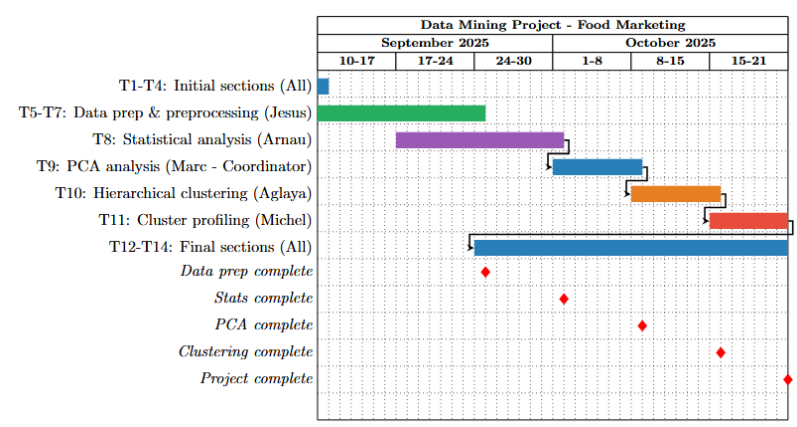
\includegraphics[width=1\linewidth]{Imatges/Gantt.png}
    \caption{Gantt Diagram for Tasks}
    \label{fig:gantt}
\end{figure}

% Legend
\begin{table}[H]
\centering
\begin{tabular}{cl}
\colorbox{JesusGreen}{\phantom{XX}} & Jesus Garcia Ayala - Data preparation \\[0.2cm]
\colorbox{ArnauPurple}{\phantom{XX}} & Arnau Hernández Navarro - Statistical analysis \\[0.2cm]
\colorbox{MarcBlue}{\phantom{XX}} & Marc Font I Cabarrocas - PCA analysis \& \textbf{Project Coordinator} \\[0.2cm]
\colorbox{AglayaOrange}{\phantom{XX}} & Aglaya Khalipskaya Soboleva - Hierarchical clustering \\[0.2cm]
\colorbox{MichelRed}{\phantom{XX}} & Alex Michel Mediavilla Jiménez - Cluster profiling \\[0.2cm]
\colorbox{SharedBlue}{\phantom{XX}} & All team members - Shared responsibilities \\
\end{tabular}
\end{table}


\textbf{\textcolor{secondaryblue}{Task Dependencies:}}
\begin{itemize}[leftmargin=*]
    \item T8 (Statistical analysis) depends on completion of T5-T7 (Data preprocessing)
    \item T9 (PCA analysis) depends on T8 completion 
    \item T10 (Hierarchical clustering) depends on T9 completion
    \item T11 (Cluster profiling) depends on T10 completion
    \item T12-T14 (Final sections) run in parallel but require integration of all analyses
\end{itemize}

\textbf{\textcolor{secondaryblue}{Critical Path:}} T5-T7 → T8 → T9 → T10 → T11 (Total: 48 days including overlaps)

\newpage
\subsection{Risk Contingency Plan}

The following risk assessment identifies potential project challenges and establishes prevention and management strategies:

\begin{table}[H]
\centering
\tiny
\renewcommand{\arraystretch}{1.3}
\begin{tabular}{|p{2.8cm}|p{3.2cm}|p{3.8cm}|p{3.8cm}|}
\hline
\rowcolor{primaryblue!10}
\textbf{\textcolor{primaryblue}{Risk}} & \textbf{\textcolor{primaryblue}{Description}} & \textbf{\textcolor{primaryblue}{How to Prevent}} & \textbf{\textcolor{primaryblue}{How to Manage}} \\
\hline
\textbf{Team Member Unavailability} & Member becomes unavailable due to illness or personal issues & Regular communication, backup assignments for critical tasks & Redistribute work among remaining members, Jesus provides technical support to any task \\
\hline
\textbf{Data Quality Issues} & Missing values, outliers, or structural problems affecting analysis validity & Early data exploration, comprehensive preprocessing planning, document assumptions & Apply robust methods, imputation techniques, transformations. Document all decisions and impacts \\
\hline
\textbf{Technical Difficulties} & Software issues, R package conflicts, computational limitations & Test packages early, ensure compatible versions, backup environments & Use alternative tools (Python), simplify models, apply sampling techniques \\
\hline
\textbf{Analysis Method Limitations} & PCA/clustering methods unsuitable for dataset characteristics & Verify assumptions early, plan alternative methods (factor analysis, different algorithms) & Switch to non-parametric methods, apply transformations, document unsuitability reasons \\
\hline
\textbf{Time Management} & Tasks exceed estimated duration, especially complex analyses & Buffer time in schedule, early start of critical tasks, regular monitoring & Prioritize essential analyses, simplify sections, redistribute completed work \\
\hline
\textbf{Integration Challenges} & Difficulty combining PCA and clustering results coherently & Plan integration strategy early, common framework, regular team meetings & Focus on significant results, use visual methods, accept contradictions with discussion \\
\hline
\textbf{Report Quality} & Poor synthesis, unclear writing, insufficient analysis depth & Early writing assignments, multiple review cycles, detailed outlines & Peer review process, clarity focus, visual aids support \\
\hline
\textbf{Data Access Delays} & Late dataset availability or understanding & Confirm access early, request documentation in advance & Use similar public datasets, adjust scope, focus on methodological rigor \\
\hline
\end{tabular}
\caption{{Risk Assessment and Mitigation Strategies}}
\label{tab:risks}
\end{table}

\textbf{\textcolor{secondaryblue}{Task Assignment Grid:}}

\begin{table}[H]
\centering
\footnotesize
\renewcommand{\arraystretch}{1.2}
\begin{tabular}{|p{3cm}|c|c|c|c|c|}
\hline
\rowcolor{primaryblue!10}
\textbf{\textcolor{primaryblue}{Task}} & \textbf{\textcolor{primaryblue}{Jesus}} & \textbf{\textcolor{primaryblue}{Arnau}} & \textbf{\textcolor{primaryblue}{Marc}} & \textbf{\textcolor{primaryblue}{Aglaya}} & \textbf{\textcolor{primaryblue}{Michel}} \\
\hline
T1-T4: Initial sections & \textcolor{primaryblue}{\textbf{X}} & \textcolor{primaryblue}{\textbf{X}} & \textcolor{primaryblue}{\textbf{X}} & \textcolor{primaryblue}{\textbf{X}} & \textcolor{primaryblue}{\textbf{X}} \\
\hline
\rowcolor{lightgray!10}
T5-T7: Data prep & \textcolor{primaryblue}{\textbf{X}} & & & & \\
\hline
T8: Statistical analysis & & \textcolor{primaryblue}{\textbf{X}} & & & \\
\hline
\rowcolor{lightgray!10}
T9: PCA analysis & & & \textcolor{primaryblue}{\textbf{X}} & & \\
\hline
T10: Clustering & & & & \textcolor{primaryblue}{\textbf{X}} & \\
\hline
\rowcolor{lightgray!10}
T11: Profiling & & & & & \textcolor{primaryblue}{\textbf{X}} \\
\hline
T12-T14: Final sections & \textcolor{primaryblue}{\textbf{X}} & \textcolor{primaryblue}{\textbf{X}} & \textcolor{primaryblue}{\textbf{X}} & \textcolor{primaryblue}{\textbf{X}} & \textcolor{primaryblue}{\textbf{X}} \\
\hline
\end{tabular}
\caption{\textcolor{primaryblue}{Task Assignment and Coordination Matrix}}
\label{tab:assignments}
\end{table}



\newpage
\section{Metadata}
\foreach \i in {1,...,8}{%
    \begin{figure}[H]
        \centering
        \includegraphics[width=\textwidth]{Imatges/metadata\i.png}
    \end{figure}
}

\newpage
\section{Preprocessing}

These are the steps we followed to carry out the preprocessing of the data. The goal of this stage is to clean, transform, and prepare the dataset, ensuring that it is consistent, reliable, and ready for the subsequent data mining tasks.

\subsection{Step 1: Getting data}
The source of the dataset used in our project comes from kaggle.com, an online platform that provides datasets, competitions, and tools for data science and machine learning. Our dataset focuses on marketing data, which will be analyzed to extract valuable insights.

\subsection{Step 2: Visualizing data}
To visualize our data, we represented it using different types of graphs, in addition to the metadata from the previous section.

\subsection{Step 3: Filtering variables selection}

 To make them easier to see and understand, we had to transform or rename a lot of variables.\\

- Age Calculation: ifood\$Age <- 2020 - ifood\$Year\_Birth creates a new column Age by subtracting the Year\_Birth from the year 2020. The original Year\_Birth column is then dropped to avoid data redundancy.\\
- Days as a Customer: ifood\$CustDays <- as.numeric(reference\_date - as.Date(ifood\$Dt\_Customer, format="\%Y-\%m-\%d")) calculates the number of days a customer has been registered. It subtracts the customer's registration date (Dt\_Customer) from a set reference\_date (December 31, 2020), converting a date variable into a useful numerical one. The original Dt\_Customer column is also removed.\\

Finally, we shortened most variable names to make them easier to represent in graphs, tables, etc.

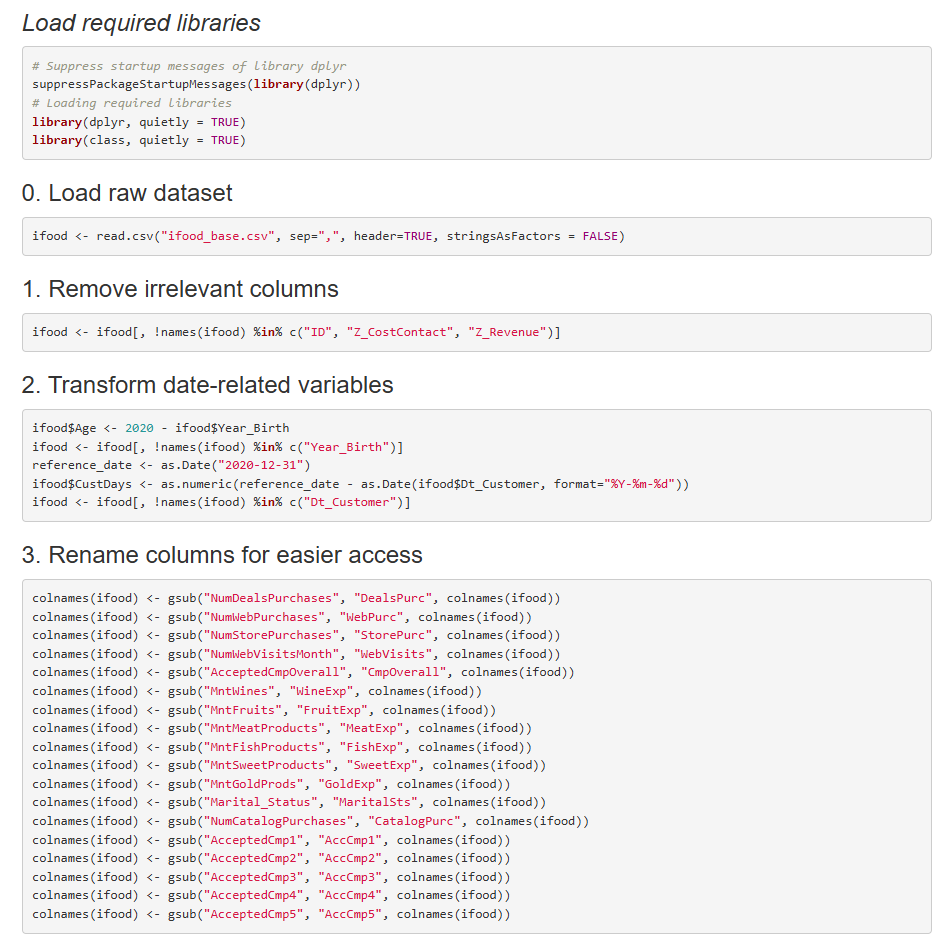
\includegraphics[width=\textwidth]{Imatges/pre1.png}

\subsection{Step 4: Missing detection and treatment}
During the preprocessing stage, we identified missing or inconsistent values by visually exploring the data to detect anomalies. For instance, in the variable Marital\_Status we found incorrect responses such as 'YOLO' and 'Absurd', which we removed to ensure data consistency.\\

Due to the fact that the Income cannot be less than 12500, we have had to impute the missing values using the KNN method.\\

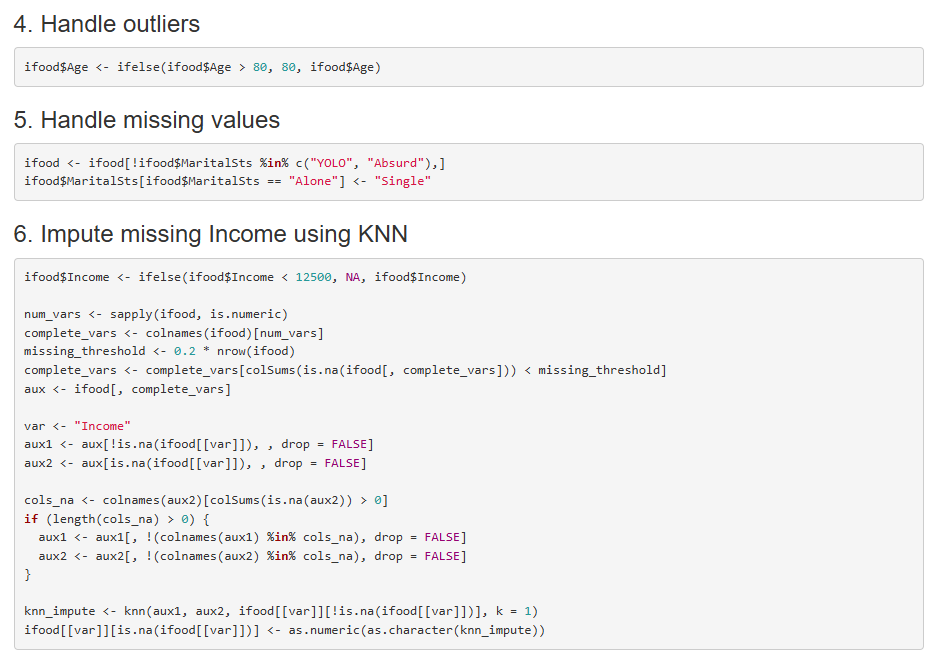
\includegraphics[width=\textwidth]{Imatges/pre2.png}
\subsection{Step 5: Outlier detection and treatment}
To handle the outliers with older people, we decided to set a limit of 80 years for individuals, so that anyone older than that age is included in the 80-year-old group.

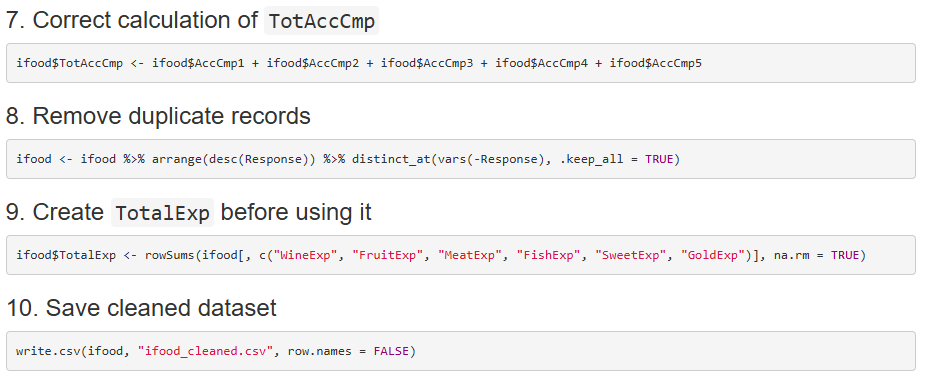
\includegraphics[width=\textwidth]{Imatges/pre3.png}
\subsection{Step 6: Feature selection}
 To clean our variables we decided to remove irrelevant columns:\\
 - ID: The ID column is a unique identifier for each record. It does'nt provide predictive value or relevant information about customer behavior or characteristics.\\
 - Z\_CostContact and Z\_Revenue: Columns starting with the letter 'Z' are often metadata variables used internally in a database, usually represents auxiliary metrics or internal calculations that are not useful for predictive analysis. In this case, both are synthetic or aggregated variables, likely related to internal company costs and revenues, which are not relevant to understanding customer behavior. \\
 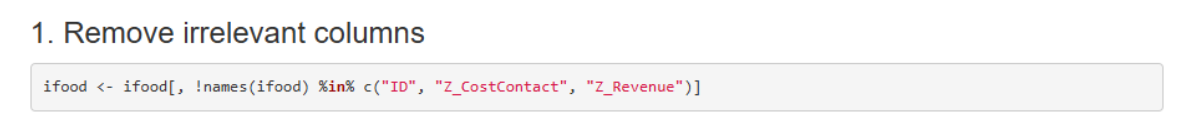
\includegraphics[width=\textwidth]{Imatges/pre8.png}
\subsection{Step 7: Transformation and new variables}
These are the new variables we have created or modified from the existing ones to obtain new information.\\
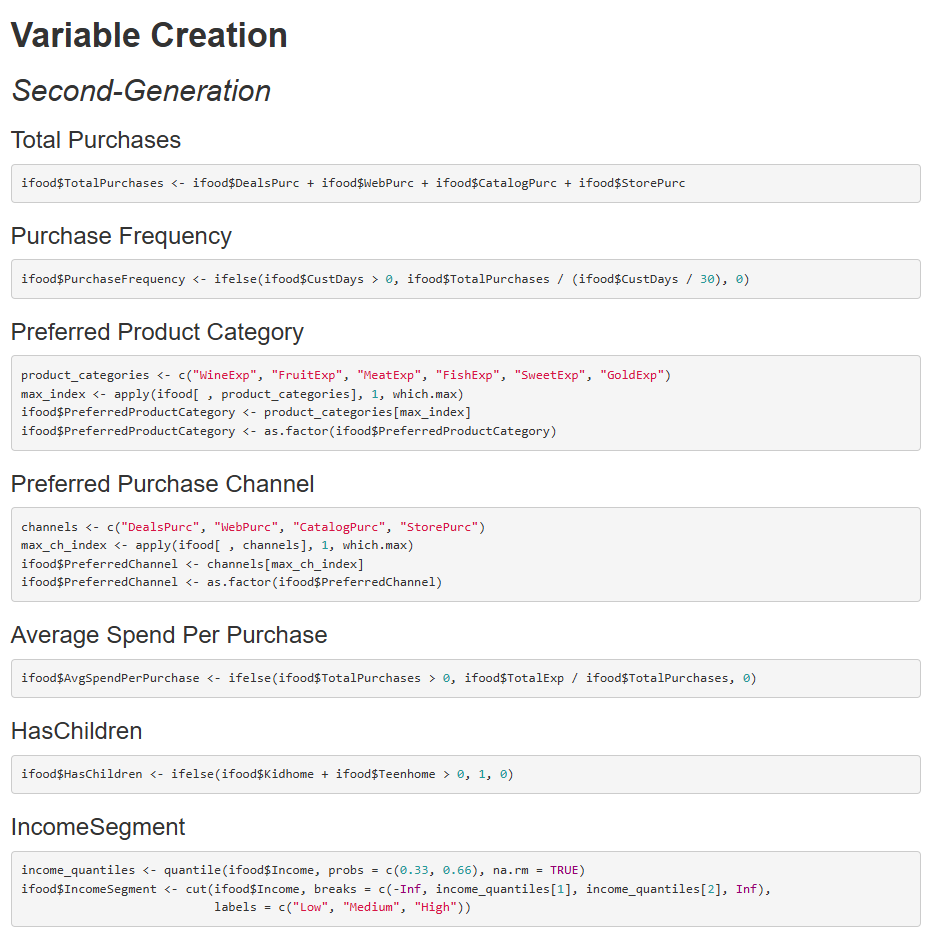
\includegraphics[width=\textwidth]{Imatges/pre4.png}

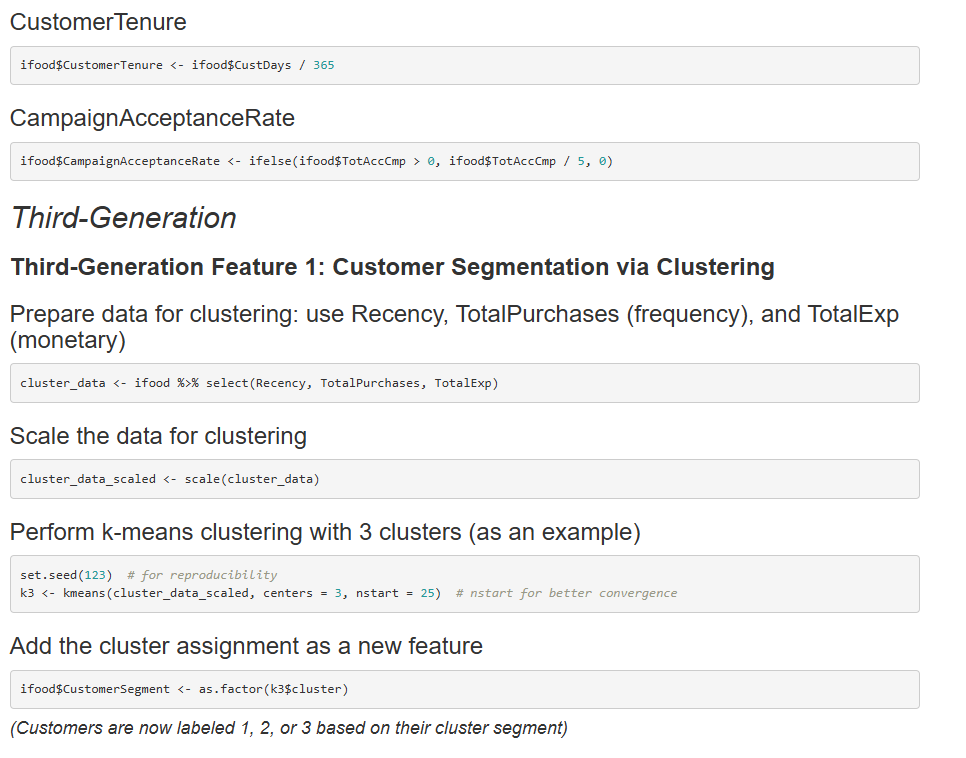
\includegraphics[width=\textwidth]{Imatges/pre5.png}
\centering
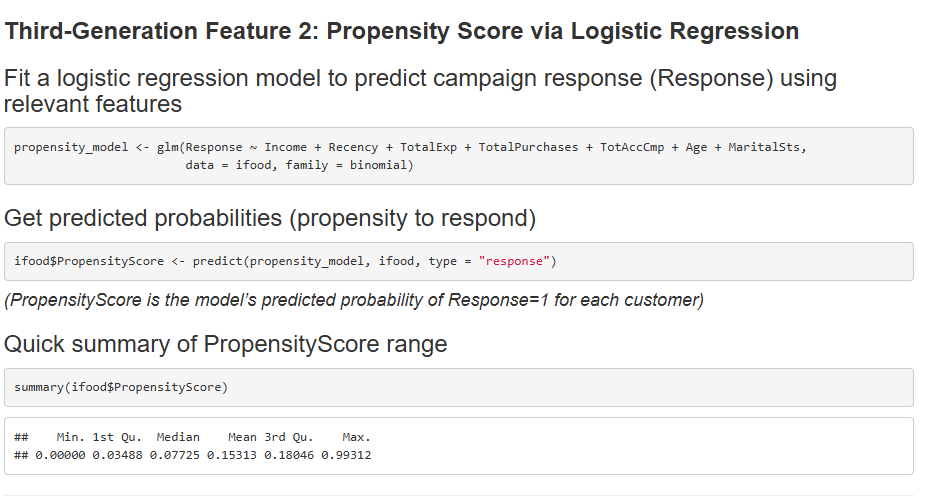
\includegraphics[width=\textwidth]{Imatges/pre6.png}
\centering
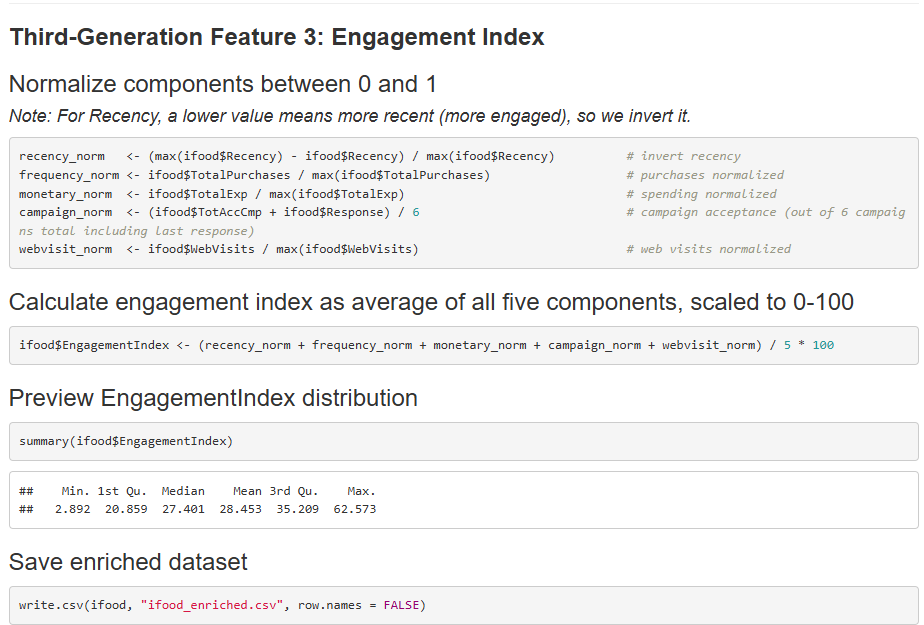
\includegraphics[width=\textwidth]{Imatges/pre7.png}

\newpage
\section{Basic Initial Univariate Descriptive Statistics of Raw Variables}
\foreach \i in {1,...,61}{%
    \begin{figure}[H]
        \centering
        \includegraphics[width=\textwidth]{Imatges/des\i.png}
    \end{figure}
}

\end{document}